% Created 2019-04-17 Mi 10:39
% Intended LaTeX compiler: pdflatex
\documentclass[presentation]{etp-beamer-fancy}
\usepackage[utf8]{inputenc}
\usepackage[T1]{fontenc}
\usepackage{graphicx}
\usepackage{grffile}
\usepackage{longtable}
\usepackage{wrapfig}
\usepackage{rotating}
\usepackage[normalem]{ulem}
\usepackage{amsmath}
\usepackage{textcomp}
\usepackage{amssymb}
\usepackage{capt-of}
\usepackage{hyperref}
\usepackage{physics}
\usepackage{siunitx}
\usepackage{booktabs}
\usepackage{microtype}
\usetheme{default}
\author{Michael Eliachevitchg}
\date{April 2019}
\title{Informal Introduction to Tracking in HEP}
\subtitle{KSETA/GK Workshop}
\institute{ETP -- KIT}
\hypersetup{
 pdfauthor={Michael Eliachevitchg},
 pdftitle={Informal Introduction to Tracking in HEP},
 pdfkeywords={},
 pdfsubject={},
 pdfcreator={Emacs 26.1 (Org mode 9.2)}, 
 pdflang={English}}
\begin{document}

\maketitle
\section*{Slides}
\label{sec:orgab95d13}
\begin{frame}[label={sec:org387b453}]{What is tracking and why do we need it?}
\begin{column}{0.6\columnwidth}
\begin{itemize}
\item HEP accelerator: produce particles in collisions
\item goal: reconstruct physically meaningful particle properties and event topology
\begin{itemize}
\item energy, momentum-vector, primary and secondary vertices, dE/dXn (\(\rightarrow\) type;)
\end{itemize}
\item tracking detectors: measure ionization from charged particles (stable: e, \(\mu\),
K, \(\pi\), p)
\item track reconstruction (tracking):
\begin{itemize}
\item find tracks (pattern recognition)
\item extract parameters (fitting)
\end{itemize}
\end{itemize}
\end{column}
\begin{column}{0.4\columnwidth}
\begin{center}
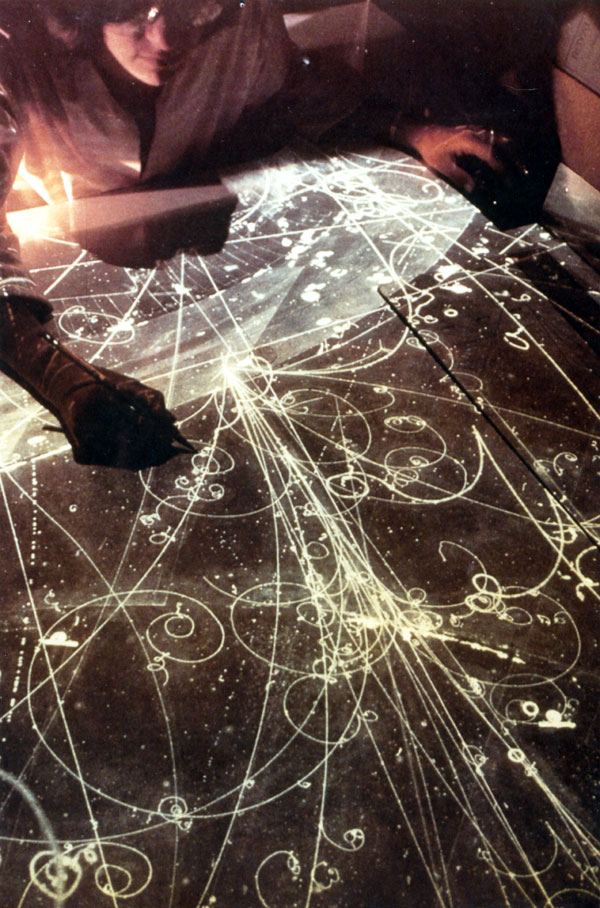
\includegraphics[width=.9\linewidth]{./figures/fermilab_bubble_chamber_scanner.jpg}
\end{center}
\end{column}
\end{frame}
\begin{frame}[label={sec:org4f28c85}]{What we measure}
\begin{itemize}
\item energy depositions: "hits"
\item 2D measurements: pixel detectors
\item 1D measurements: strip detectors, wire chamber (measurements are times)
\item binary or non-binary information (useful for dE/dX, weighting)
\end{itemize}
\end{frame}
\begin{frame}[label={sec:org244e137}]{Why is difficult? Example: (HL)-LHC}
\begin{itemize}
\item pile-up and underlying event \(\rightarrow\) large number of tracks from IP
\begin{itemize}
\item combinatorics + ambiguities
\end{itemize}
\item lumi + large cross section \(\rightarrow\) high event rate \(\rightarrow\) little time per event
\item HLLHC: current CPU-time surpasses computing budget
\begin{itemize}
\item faster algorithms required
\end{itemize}
\end{itemize}
\begin{columns}
\begin{column}{0.5\columnwidth}
\begin{center}
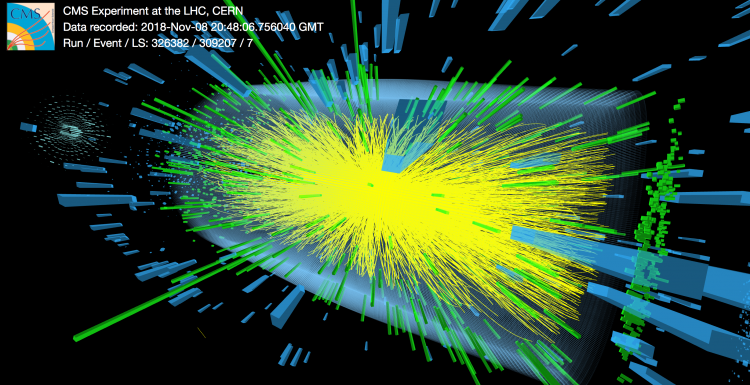
\includegraphics[width=.9\linewidth]{./figures/cms_heavy_ion_eventdisplay.png}
\end{center}
\end{column}
\begin{column}{0.5\columnwidth}
\begin{center}
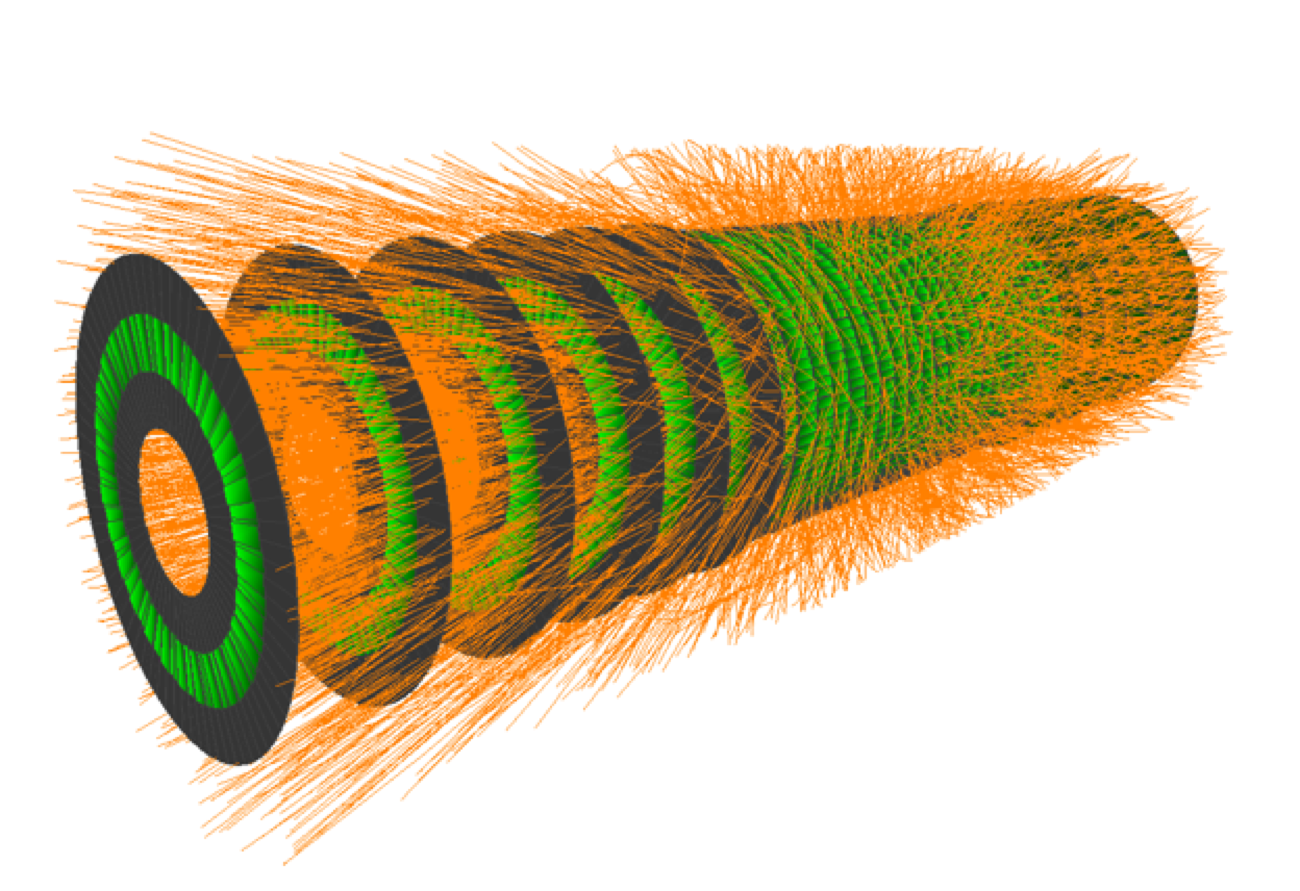
\includegraphics[width=.9\linewidth]{./figures/trackml_generic_detector.png}
\end{center}
\end{column}
\end{columns}
\end{frame}
\begin{frame}[label={sec:orge8cf8c9}]{Interlude: Belle II}
\begin{itemize}
\item e\textsuperscript{+}e\textsuperscript{-} B-factory operating on the Y(4S) resonance at 11.58 GeV
\item asymmetric beam energies to resolve B decay vertices
\end{itemize}
\begin{columns}
\begin{column}{0.6\columnwidth}
\begin{center}
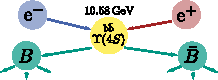
\includegraphics[width=.5\textwidth]{./figures/eplus_eminus_to_b_bar_diagram.pdf}
\end{center}
\begin{center}
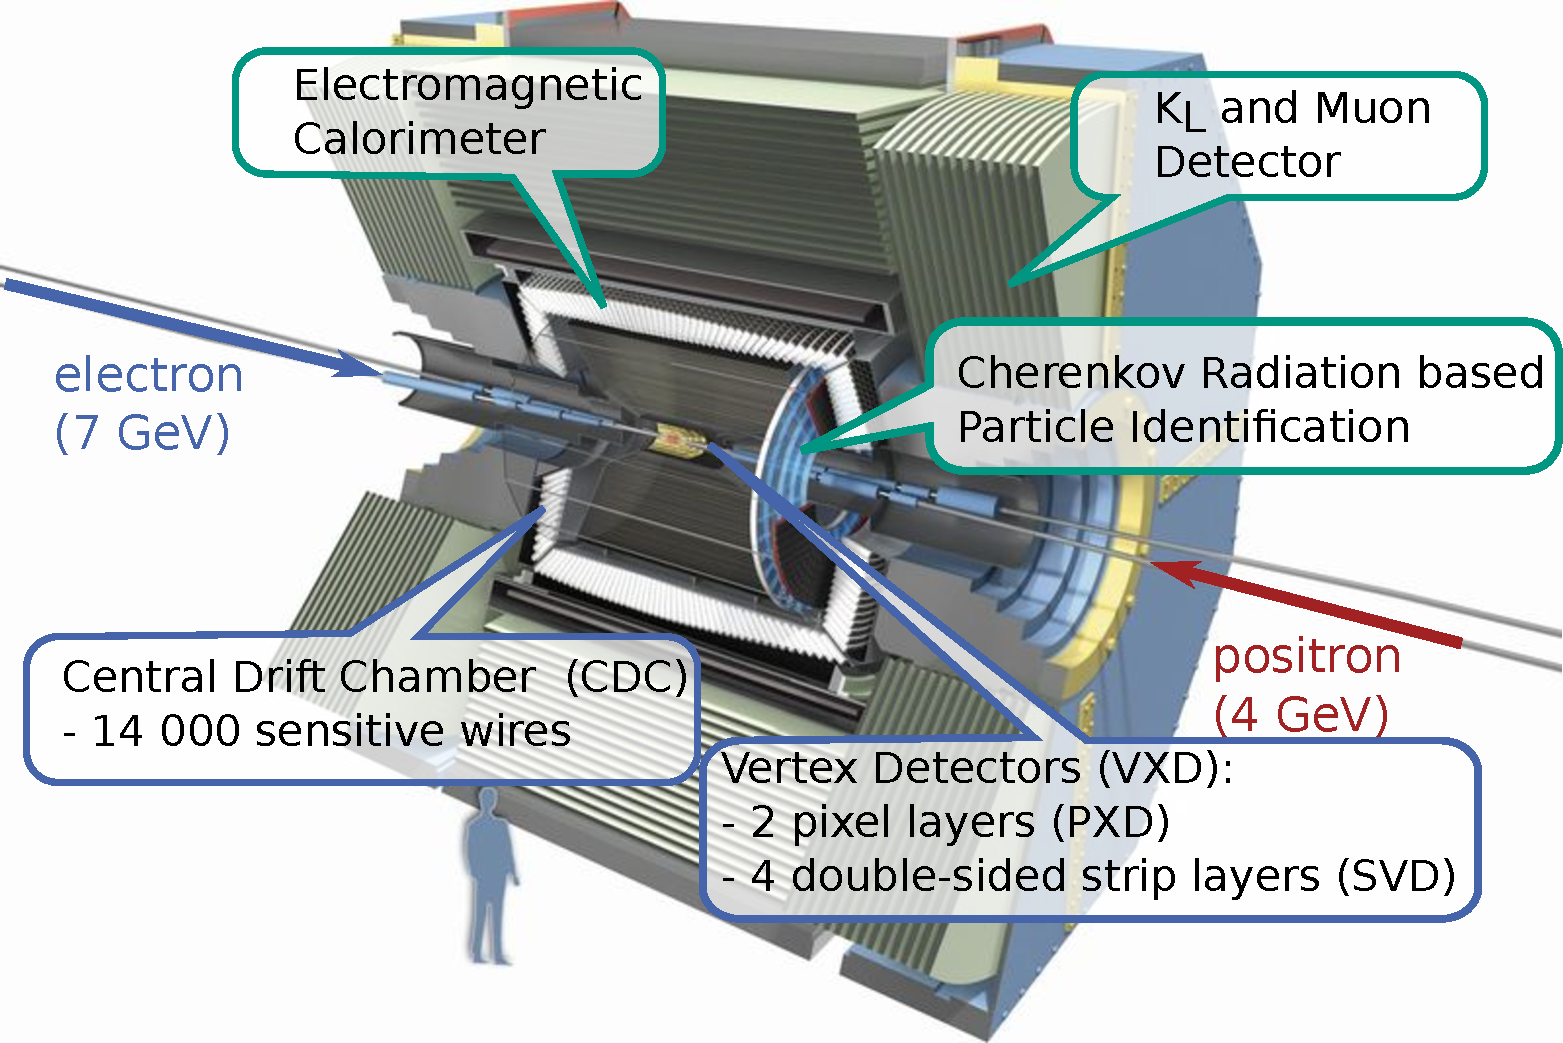
\includegraphics[width=\textwidth]{./figures/belle2_detector_dpgaachen.pdf}
\end{center}
\end{column}
\begin{column}{0.4\columnwidth}
\begin{center}
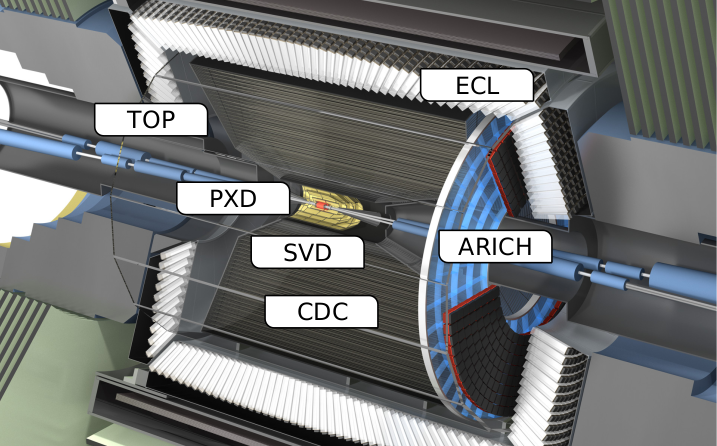
\includegraphics[width=.9\linewidth]{./figures/belle2_detector_trackingzoom.png}
\end{center}
\end{column}
\end{columns}
\end{frame}
\begin{frame}[label={sec:org169fa11}]{Tracking subdetectors}
\begin{columns}
\begin{column}{0.5\columnwidth}
\begin{center}
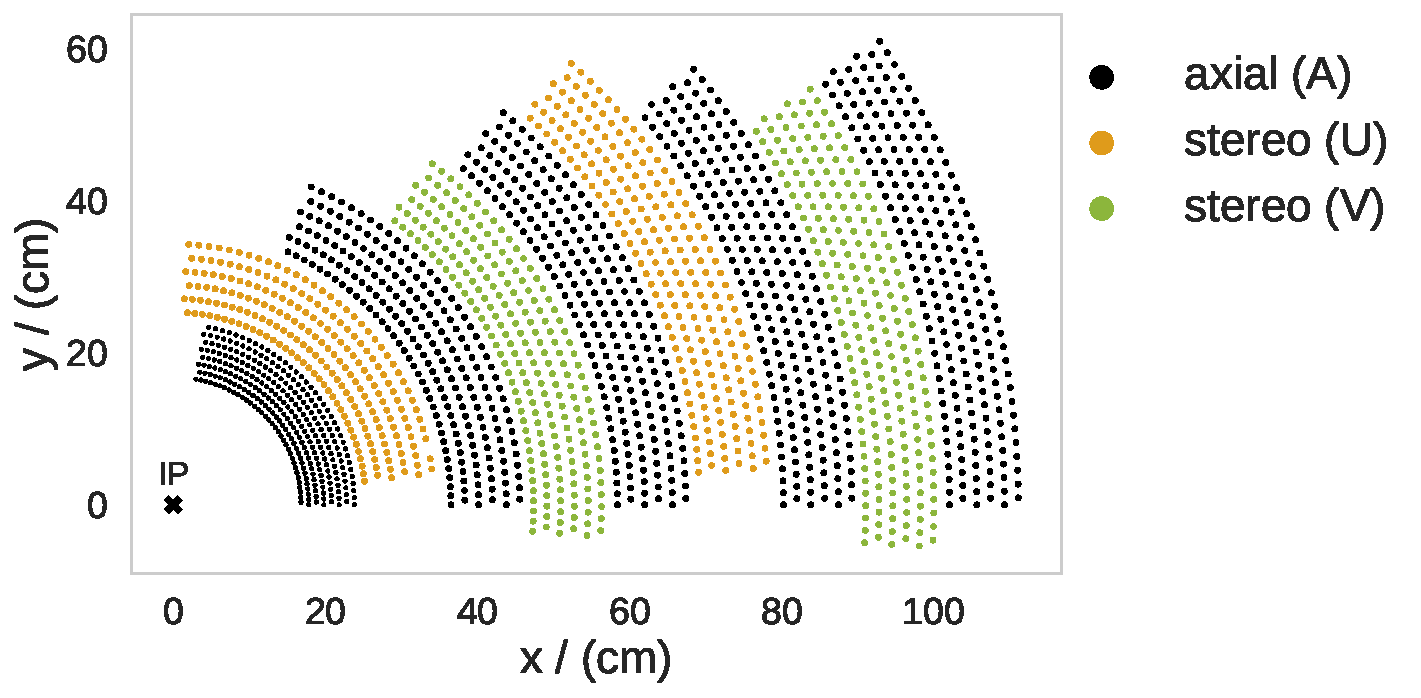
\includegraphics[width=.9\linewidth]{./figures/my_cdc_wire_configuration_plot.pdf}
\end{center}
\begin{columns}
\begin{column}{0.35\columnwidth}
\begin{center}
\includegraphics[width=.9\linewidth]{./figures/axial_layer_cropped.pdf}
\end{center}
\end{column}
\begin{column}{0.35\columnwidth}
\begin{center}
\includegraphics[width=.9\linewidth]{./figures/stereo_layer_hyperboloid_cropped.pdf}
\end{center}
\end{column}
\end{columns}
\end{column}
\begin{column}{0.5\columnwidth}
\begin{center}
\includegraphics[width=.9\linewidth]{./figures/vxd_layers_labelled.png}
\end{center}
\begin{center}
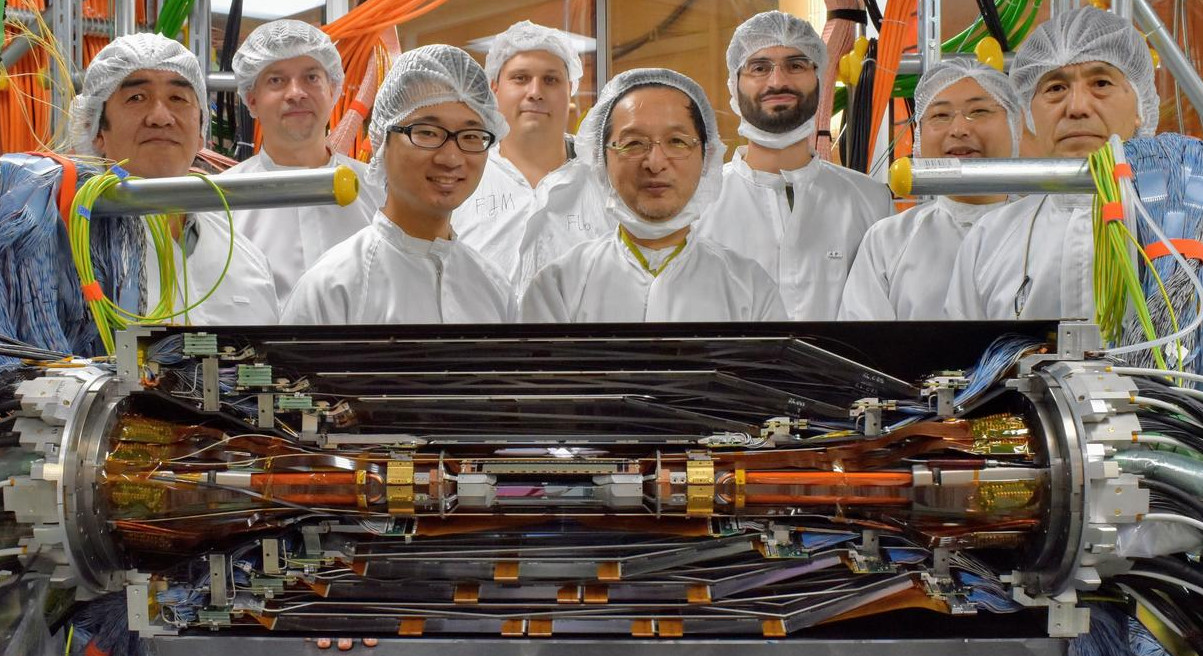
\includegraphics[width=.9\linewidth]{./figures/vertexdetector_cropped.jpg}
\end{center}
\end{column}
\end{columns}
\end{frame}

\begin{frame}[label={sec:org32d6934}]{Why is difficult? Example: Belle II}
\begin{itemize}
\item Y(4S) decays: only \alert{11 tracks} per event
\item high luminosity \(\rightarrow\) large beam-induced background
\begin{itemize}
\item PXD: \alert{10\textsuperscript{4} backkground hits} expected
\end{itemize}
\item \(\sqrt{s} = 10.58 GeV\): \alert{low-momentum} tracks
\item curl in tracking system
\item scattering significant
\item physics analyzes: require reconstruction of whole event
\end{itemize}
\end{frame}
\begin{frame}[label={sec:orgb75ba41}]{How I learned it}
\begin{columns}
\begin{column}{0.6\columnwidth}
\begin{itemize}
\item curvature in B-field allows momentum estimation
\item \(p_T = \frac{R}{qB}\), \(p_T = p \cos{theta}\)
\item estimate curvature from sagitta s
\end{itemize}
\begin{center}
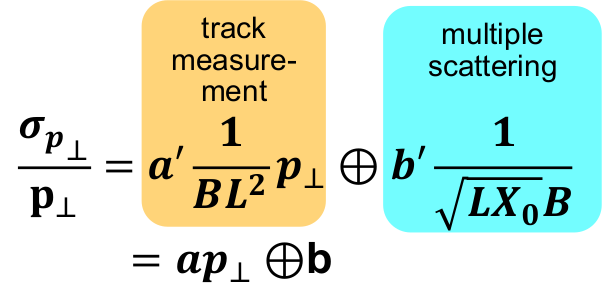
\includegraphics[width=.5\textwidth]{./figures/tracking_uncertainty_hartmann.png}
\end{center}
\end{column}
\begin{column}{0.4\columnwidth}
\begin{center}
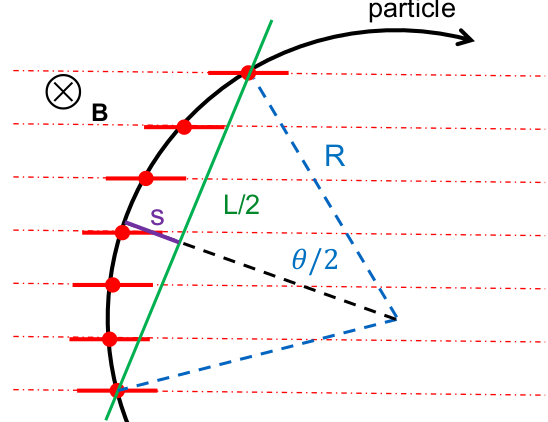
\includegraphics[width=.9\linewidth]{./figures/tracking_sagitta_hartmann.png}
\end{center}
\end{column}
\end{columns}
\end{frame}
\begin{frame}[label={sec:org6c5dc2d}]{How it's done: Local and global algorithms}
\begin{itemize}
\item global
\begin{itemize}
\item take all hits into account at the same
\item assume helical tracks from IP
\item stable with backgrounds and gaps in hit pattern
\end{itemize}
\item local
\begin{itemize}
\item build track via local relations between hits
\item can handle large scattering and tracks not from IP
\end{itemize}
\end{itemize}
\end{frame}
\begin{frame}[label={sec:orgf9b2e2d},fragile]{Legendre algorithm: Hough Transform}
 \begin{columns}
\begin{column}{.7\columnwidth}
\begin{itemize}
\item Legendre algorithm is extension of \alert{Hough Transform}
\begin{itemize}
\item transform xy-space into \(\rho \theta\)-space, where each line is represented as a point
\item \(\rho = x \cos{\theta} + y \sin{\theta}\)
\item for each point in the original space, draw all points in the \(\rho \theta\)-space
consistent with a line through through that point
\end{itemize}
\end{itemize}
;**** Algorithmus von \href{https://de.wikipedia.org/wiki/Hough-Transformation}{Wikipedia}                           :B\textsubscript{ignoreheading}:
:BEAMER\textsubscript{env}: ignoreheading
\begin{verbatim}
foreach pixel != 0:
   for theta := 0 to pi:
      rho := pixel_x * cos(theta)
             + pixel_y * sin(theta)
      houghRaum[theta][rho]++
\end{verbatim}
\end{column}
\begin{column}{0.3\columnwidth}
\begin{center}
\includegraphics[width=.9\linewidth]{./figures/deathstar_trench_src.png}
\end{center}
\begin{center}
\includegraphics[width=.9\linewidth]{./figures/deathstar_trench_dst.png}
\end{center}
\begin{center}
\includegraphics[width=.9\linewidth]{./figures/deathstar_trench_hough.png}
\end{center}
\begin{center}
\includegraphics[width=.9\linewidth]{./figures/death-star-trench-hud.png}
\end{center}
\end{column}
\end{columns}
\end{frame}
\begin{frame}[label={sec:org44be6a9}]{Legendre: Linearize circular tracks}
\begin{itemize}
\item circles through origin again described by only two parameters (in 2D)
\item do the same thing again
\end{itemize}
\begin{center}
\includegraphics[width=.7\textwidth]{./figures/legendre_inverted_plane.png}
\end{center}
\end{frame}

\begin{frame}[label={sec:org45f75a9}]{Legendre}
\begin{center}
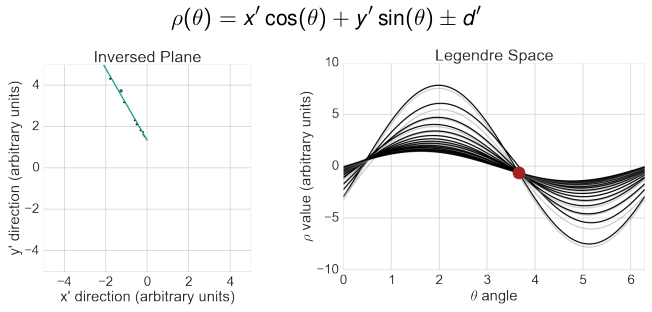
\includegraphics[width=.7\textwidth]{./figures/legendre_transform.png}
\end{center}
\end{frame}

\begin{frame}[label={sec:orgac0e8be}]{Local: Cellular Automaton}
\begin{itemize}
\item search for longest path in graph (DAG) with nodes and edges
\item length = sum of weightes edges and nodes
\item e.g. CDC: nodes are hit triplets, edges from BDT
\end{itemize}
\begin{center}
\includegraphics[width=.5\textwidth]{./figures/segment_from_triplets.png}
\end{center}
\end{frame}
\begin{frame}[label={sec:org072bfae}]{Local: Combinatorial Kalman Filter}
\end{frame}
\begin{frame}[label={sec:orgf12a813}]{How it all comes together}
\begin{center}
\includegraphics[width=.55\textwidth]{./figures/full_track_finding_simplified.pdf}
\end{center}
\end{frame}
\begin{frame}[label={sec:org6f7bd4d}]{When it works}
\begin{center}
\includegraphics[width=.5\textwidth]{./figures/b2phase3_1st_bantib_like_event_cropped.png}
\end{center}
\end{frame}
\begin{frame}[label={sec:org2523bb2}]{Extra: deep learning approaches to track finding}
\end{frame}
\end{document}